%\documentclass{acmsiggraph}                     % final
\documentclass[annualconference]{acmsiggraph}  % final (annual conference)
%\documentclass[review]{acmsiggraph}            % review
%\documentclass[widereview]{acmsiggraph}        % wide-spaced review
%\documentclass[preprint]{acmsiggraph}          % preprint

%% Uncomment one of the five lines above depending on where your paper is
%% in the conference process. ``review'' and ``widereview'' are for review
%% submission, ``preprint'' is for pre-publication, and ``final'' is for
%% the version to be printed. The ``final'' variant will accept the 
%% ``annualconference'' parameter, which changes the height of the space
%% left clear for the ACM copyright information.

%% The 'helvet' and 'times' packages define the typefaces used for
%% serif and sans serif type in this document. Computer Modern Roman 
%% is used for mathematics typesetting. The scale factor is set to .92
%% to bring the sans-serif type in line with the serif type.

\usepackage[scaled=.92]{helvet}
\usepackage{times}
\usepackage{latexsym}

%% The 'graphicx' package allows for the inclusion of EPS figures.

\usepackage{graphicx}

%% use this for zero \parindent and non-zero \parskip, intelligently.

\usepackage{parskip}

%% Optional: the 'caption' package provides a nicer-looking replacement
%% for the standard caption environment. With 'labelfont=bf,'textfont=it',
%% caption labels are bold and caption text is italic.

\usepackage[labelfont=bf,textfont=it]{caption}

%% If you are submitting a paper to the annual conference, please replace 
%% the value ``0'' below with the numeric value of your OnlineID. 
%% If you are not submitting this paper to the annual conference, 
%% you may safely leave it at ``0'' -- it will not be included in the output.

\usepackage{listings}
\usepackage{alltt}
\usepackage{subfigure}

%%\usepackage[caption=false]{subfig}

\onlineid{paper1041}

%% Paper title.

\title{Integration of X3D Geospatial in a Data Driven Web Application}

%% Author and Affiliation (single author).

%%\author{Roy G. Biv\thanks{e-mail: roy.g.biv@aol.com}\\Allied Widgets Research}

%% Author and Affiliation (multiple authors).


\author{Michael McCann\thanks{e-mail: mccann@mbari.org}\\MBARI
\and Byounghyun Yoo\thanks{e-mail: yoo@byoo.net}\\Korea Institute of Science and Technology
\and Don Brutzman\thanks{e-mail: brutzman@nps.edu}\\Naval Postgraduate School}


%% Keywords that describe your work.
\keywords{X3D, geospatial, sensor data, oceanography, X3DOM}

%%%%%% START OF THE PAPER %%%%%%

\begin{document}




%% The ``\maketitle'' command must be the first command after the
%% ``\begin{document}'' command. It prepares and prints the title block.

\maketitle

%% Abstract section.

%%%\begin{abstract}
%%%\end{abstract}

%% ACM Computing Review (CR) categories. 
%% See <http://www.acm.org/class/1998/> for details.
%% The ``\CRcat'' command takes four arguments.

\begin{CRcatlist}
\CRcat{I.3.6}{Computing Methodologies}{Computer Graphics}{Methodology and Techniques}
\end{CRcatlist}

%% The ``\keywordlist'' command prints out the keywords.
\keywordlist


\copyrightspace
%% The ``\copyrightspace'' command must be the first command after the 
%% start of the first section of the body of your paper. It ensures the
%% copyright space is left at the bottom of the first column on the first
%% page of your paper.

\section{Overview}

The Monterey Bay Aquarium Research Institute designed the Spatial Temporal Oceanographic Query System (STOQS) \cite{STOQS} to create new capabilities for scientists to gain insight from their data. STOQS employs open standards and is a 100\% free and open source project. It includes a web-based graphical user interface where X3D Geospatial has been integrated to enable 3D geospatial data visualization. 

\section{Architecture}

STOQS consists of a PostgreSQL/PostGIS database, Mapserver, and Python-Django running on a server and client-side technology (HTML5, CSS, jQuery, OpenLayers, X3DOM, Bootstrap) running in a modern web browser (Fig.~\ref{fig:STOQSArch}). The web application provides faceted search capabilities allowing a user to quickly drill into data of interest. The X3DOM JavaScript library provides interactive 3D views of the data in browsers that support WebGL.  

\begin{figure}[htbp]
\centering
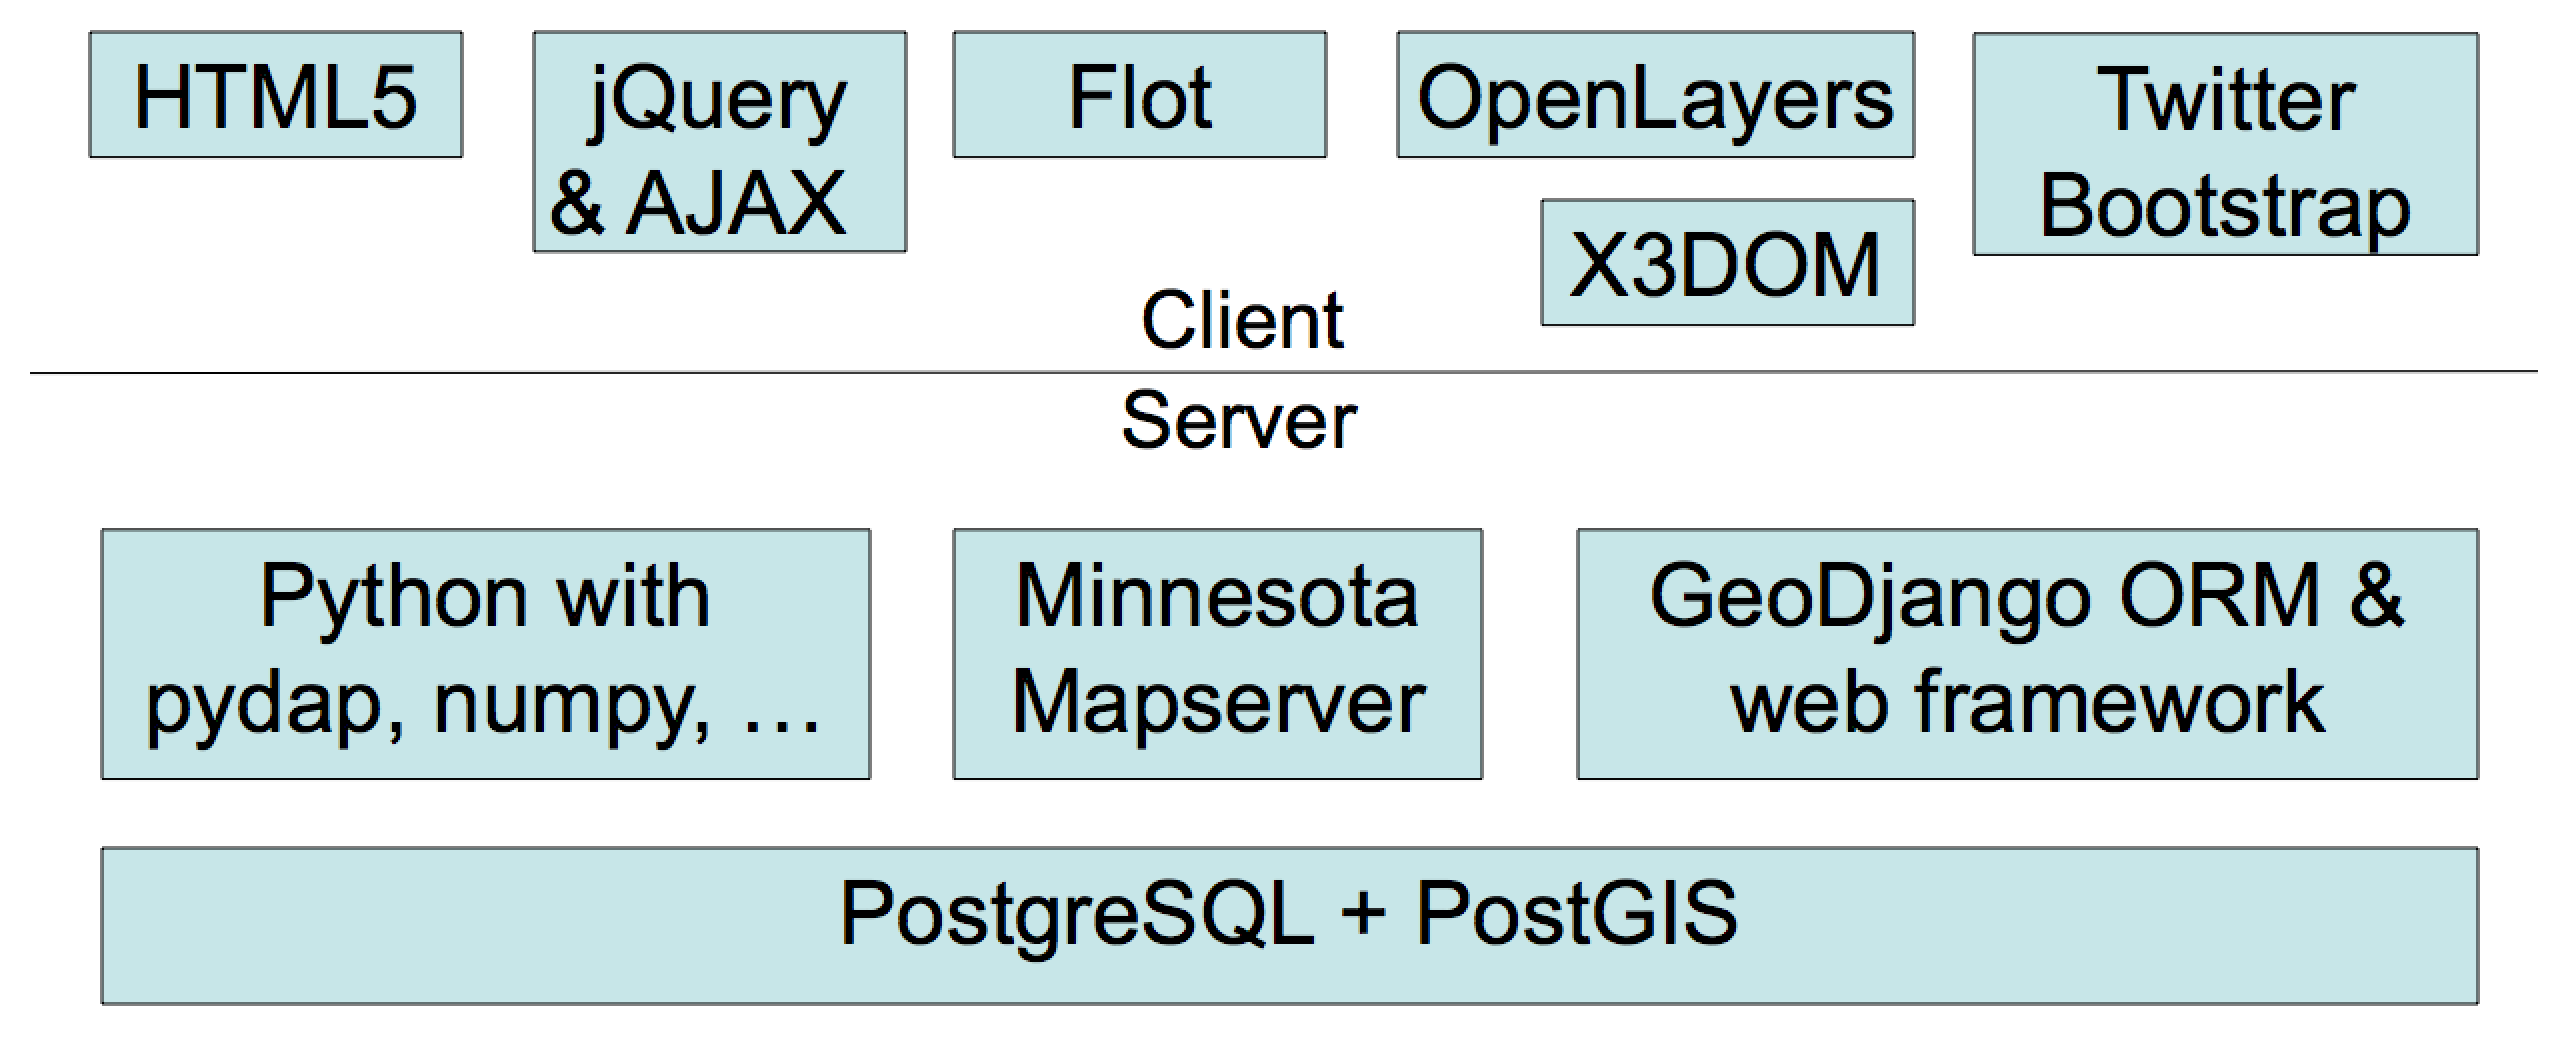
\includegraphics[width=2.7in]{stoqs_arch_simple.png}
\caption{STOQS integrates multiple open-source components.}
\label{fig:STOQSArch}
\end{figure}




\begin{figure}[htbp]
\centering
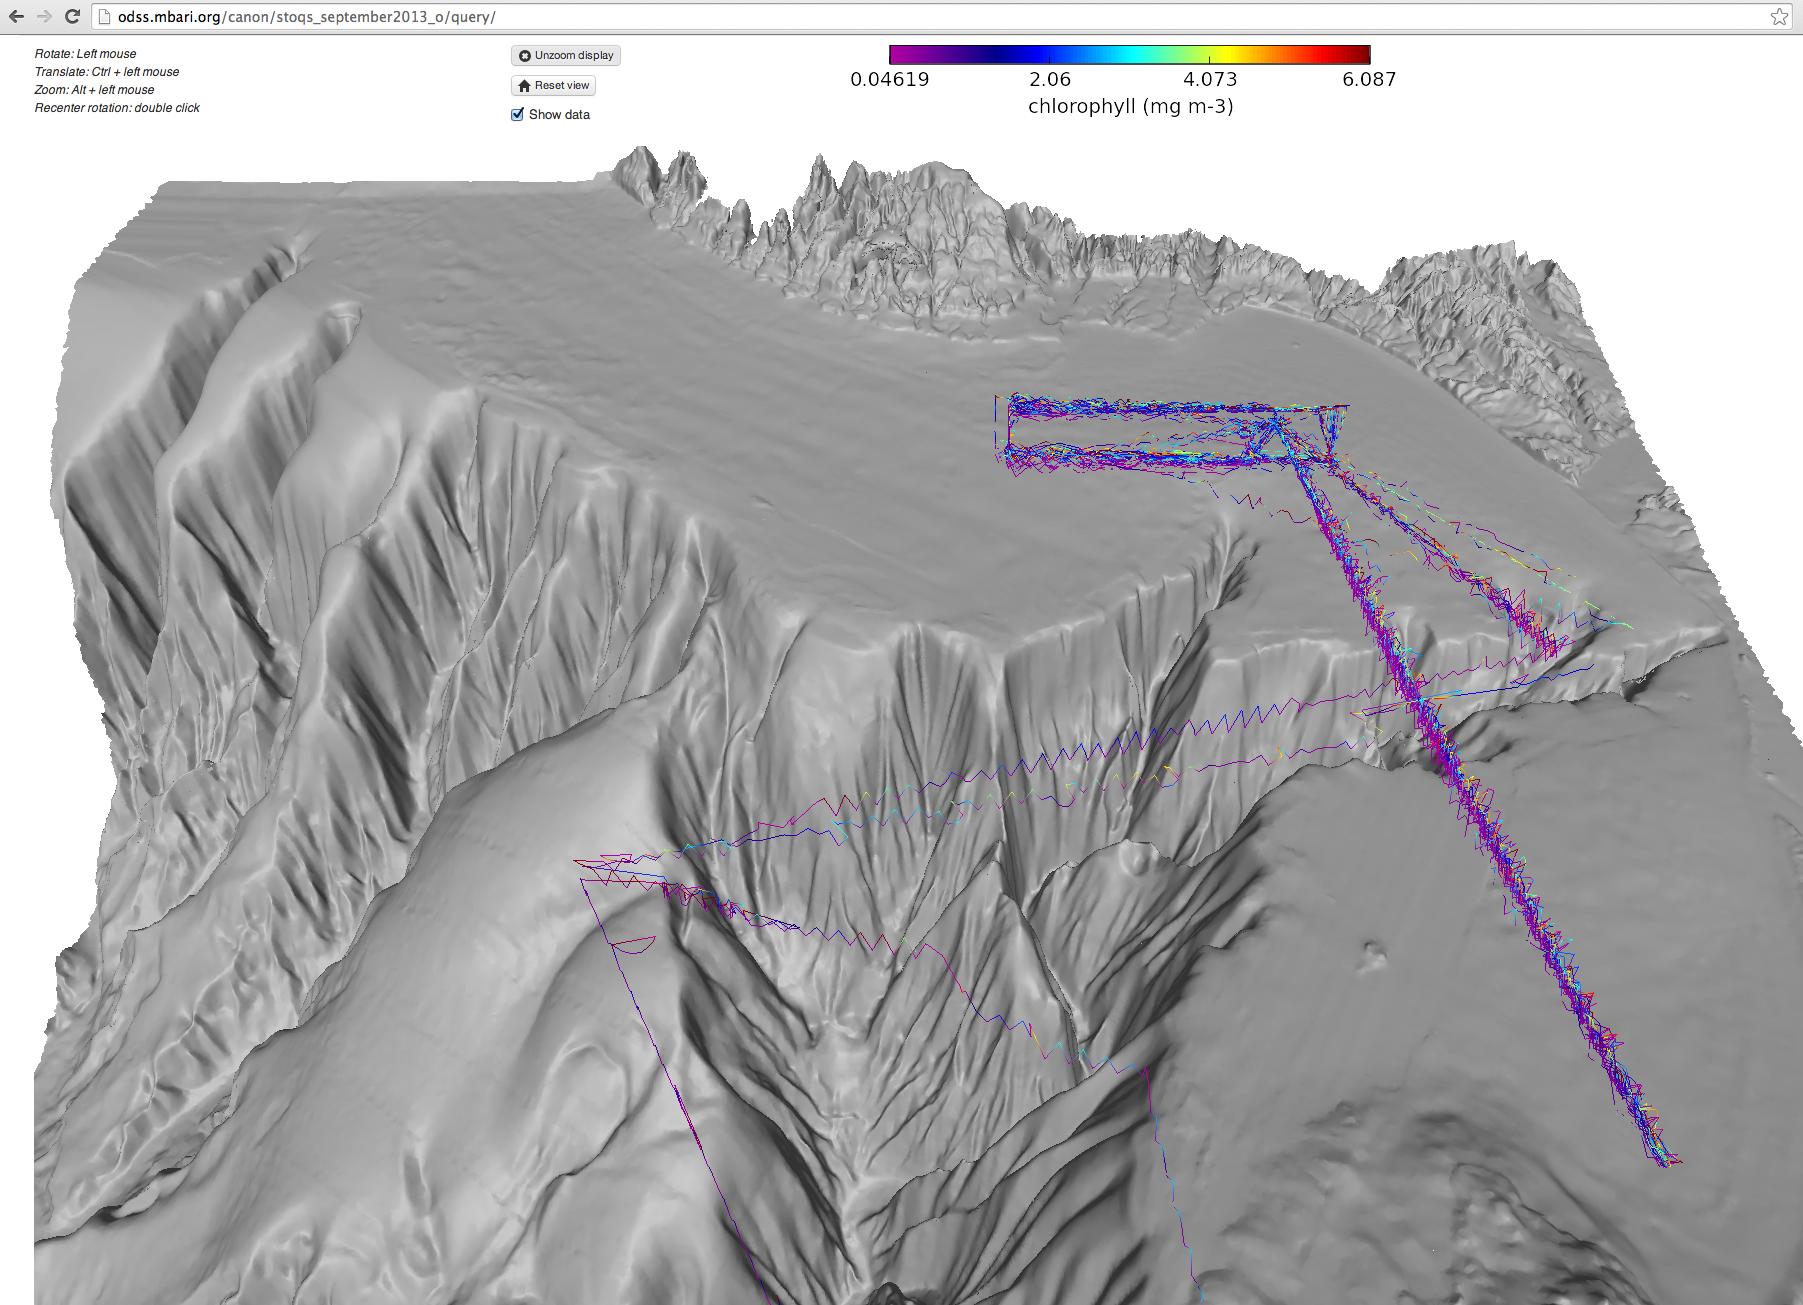
\includegraphics[width=2.8in]{Monterey25_lrauvs.png}
\caption{Chlorophyll sensor data over Monterey Bay bathymetry.}
\label{fig:Monterey25_lrauvs}
\end{figure}



\section{Discussion of geospatial standards}
STOQS is a good platform for experimentation with 3D portrayal and for understanding patterns of data access. Such experimentation helps identify needed protocols to support interoperable data access and 3D visualization.
Data from the database can be connected to appropriate scene graph elements within the confines of the coupled Server-AJAX-JSON-Client environment. For example, 
Fig.~\ref{fig:Monterey25_lrauvs} is a screen grab from the STOQS User Interface where the user has selected Autonomous Underwater Vehicle measurements of chlorophyll. The system retrieved the selected data from the database in a custom JSON data structure, JavaScript in the browser then updated IndexedLineSet GeoCoordinates in the scene graph with these data. 

The Spatial section of the STOQS UI has both 2D (OpenLayers) and 3D (X3DOM) data viewing areas. OpenLayers supports the Open Geospatial Consortium's Web Map Service (WMS) protocol which allows content to be retrieved and "mashed up" from different servers. The WMS protocol enables this through its requirement that each GetMap request include a CRS field specifying the EPSG code for the coordinate reference system of the map.  There is not yet an equivalent scheme to deliver 3D data to an X3D scene graph.

The OGC 3D Portrayal Interoperability Experiment (3DPIE) \cite{3DPIE} specifies that a GetScene request will return an entire X3D scene in whatever coordinates the server generates - there is no ability to mash up data from different servers. We think that this situation can be improved and are implementing the X3D Geospatial Component in X3DOM to explore ways to achieve fully interopable 3D portrayal.

There are several use cases for 3D mashup capability. The 3DPIE identified sensor data as a source for portrayal but left the implementation of a sensor service capability for a future effort. Data representing such things as atmospheric pollutants could be retrieved from external servers and could be portrayed as a transparent cloud within a model of a city. 
Remote sensing and numerical model data could be retrieved from other servers and rendered in 3D along with the oceanographic sensor data in STOQS.


\bibliographystyle{acmsiggraph}
\nocite{*}
\bibliography{IntegrationOfX3DGeospatialOnePage}




\end{document}
